% \begin{tikzpicture}[
    box/.style={draw, minimum width=2cm, minimum height=3cm, text width=1.8cm, align=center},
    smallbox/.style={draw, minimum width=1.5cm, minimum height=1.2cm, text width=1.8cm, align=center},
    arrow/.style={->, >=latex, thick},
    label/.style={font=\small},
    % circle/.style={draw, align=center}
]

% Components
\node[circle, draw] (input) {Input $x$};
\node[box, right=1cm of input] (encoder) {Encoder};

% Latent space
\node[right=2cm of encoder] (latent) {};
\node[circle, draw, right=1cm of encoder, font=\small, align=center,text width=2cm] (quantized) {Quantized \\ z};
\node[smallbox, below=0.3cm of quantized] (codebook) {Codebook};

\node[box, right=2cm of latent] (decoder) {Decoder};
\node[circle, draw, right=1cm of decoder] (output) {Output $\hat{x}$};

% Connections
\draw[arrow] (input) -- (encoder);
\draw[arrow] (encoder) -- (quantized);
\draw[arrow] (codebook) -- (quantized);
\draw[arrow] (quantized) -- (decoder);
\draw[arrow] (decoder) -- (output);

% Labels
\node[label, below=0.2cm of input] {High-dimensional};
\node[label, below=0.2cm of codebook] {Latent space};
\node[label, below=0.2cm of output] {Reconstructed};

% Reconstruction Loss
\draw[<->, >=latex, bend right=30] ($(input.south west)+(1,-0.3)$) to node[below, font=\small] {Reconstruction Loss} ($(output.south east)+(-1.3,-0.2)$);

% Commitment Loss
\draw[<->, >=latex, bend left=40] ($(encoder.north east)+(0.2,0.2)$) to node[above=0.1cm, font=\small] {Commitment Loss} ($(quantized.north west)+(-0.2,0.2)$);

\end{tikzpicture}
\begin{figure}[H]
    \centering
    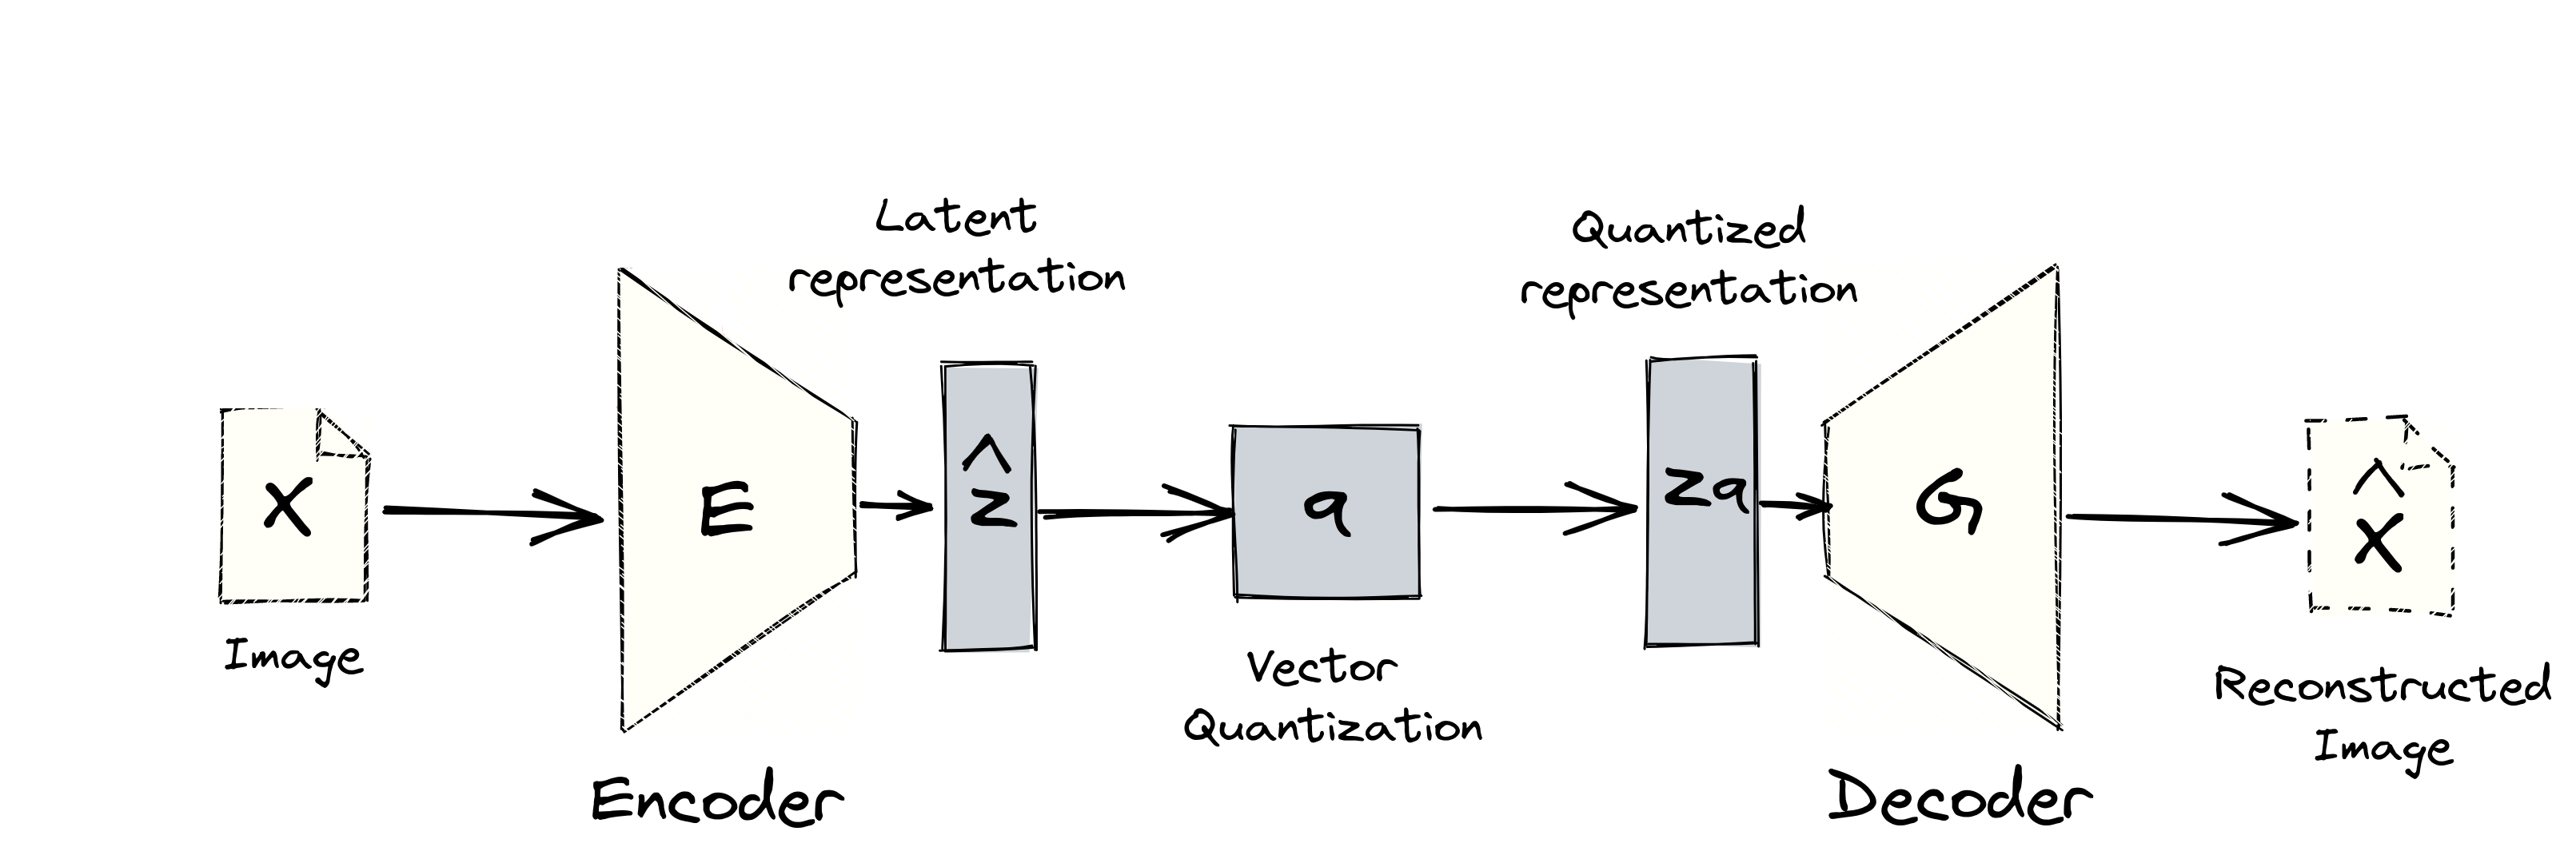
\includegraphics[width=\linewidth]{concept_engineering/vqgan/vqvae.png}
    \caption{Visualization of Vector Quantized Variational Autoencoder\cite{miranda2021vqgan}.}
    \label{fig:vavae1}
\end{figure}

The latent representation of the variational autoencoders $z$ is close to $\sim \mathbb{N}(0,1)$. Unfortunately, it sometimes leads to posterior collapse. This means that the decoder starts to treat latent representation $z$ as meaningless noise and ignores it. Instead, it learns to encode the dataset in itself. When something like this happens, the decoder cannot generate meaningful results, no matter the given $z$. 

\begin{figure}[H]
    \centering
    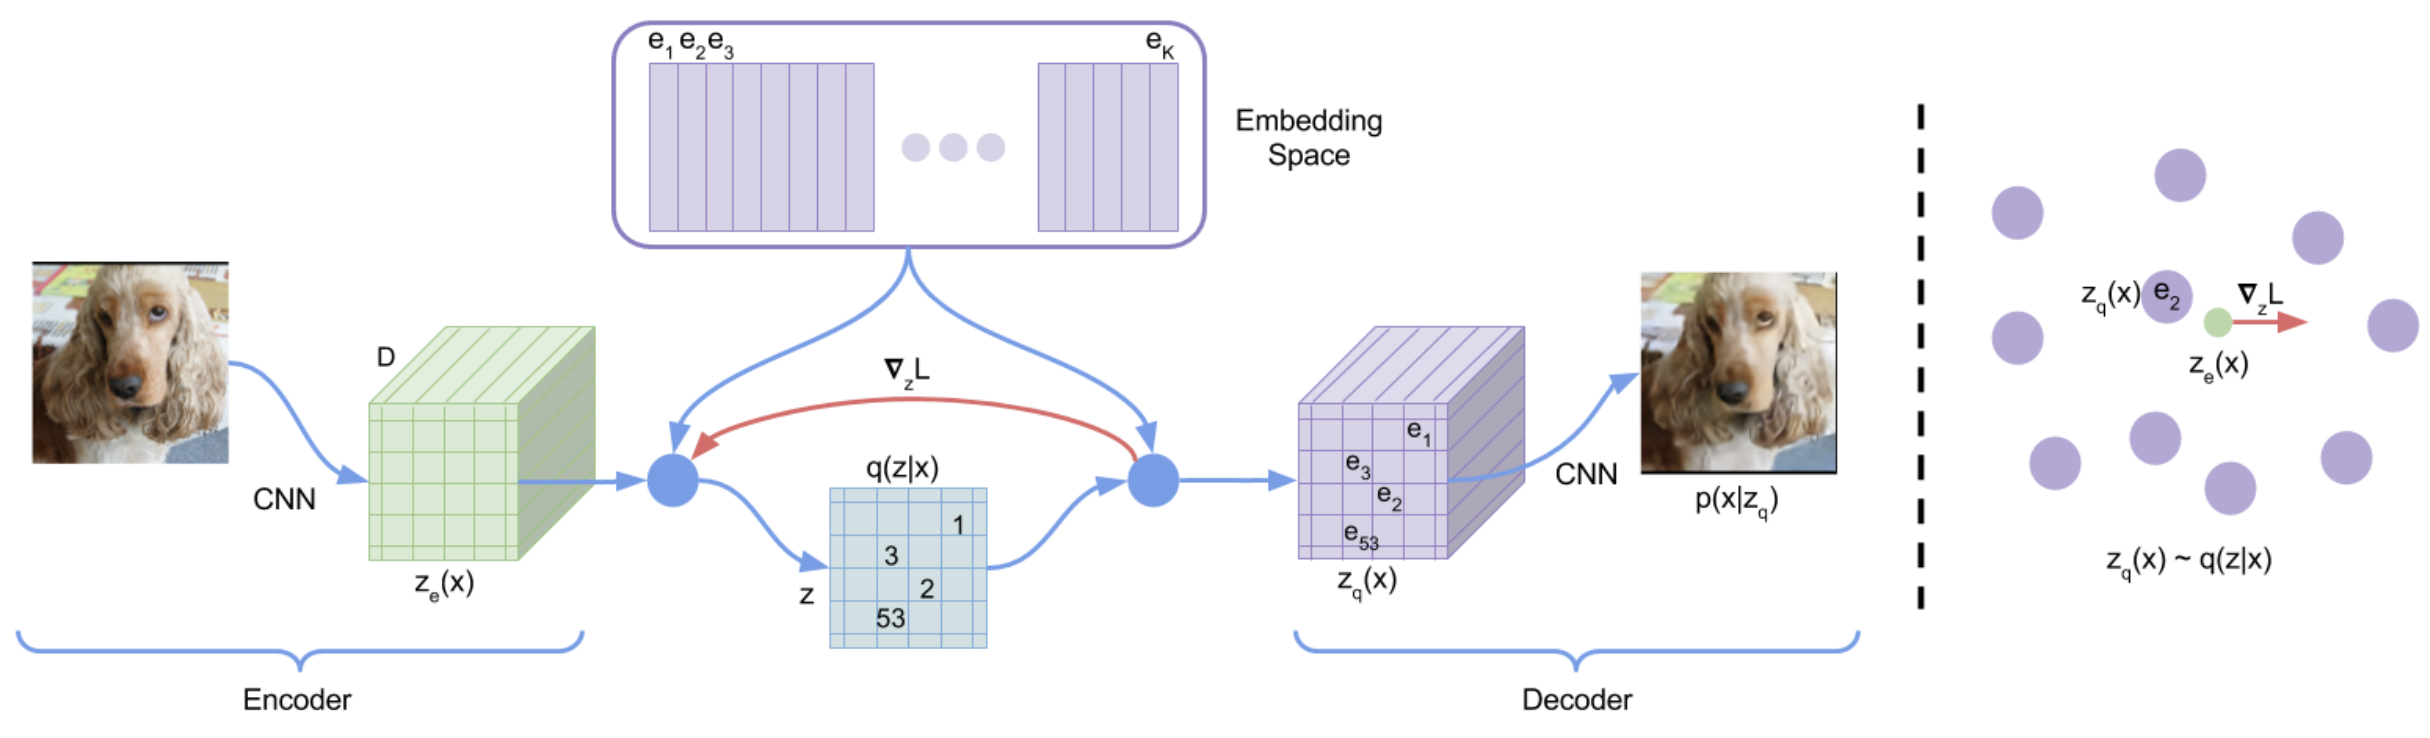
\includegraphics[width=\linewidth]{concept_engineering/vqvae.png}
    \caption{VQVAE visualization showing compression of an image to latent representation (a cube), encoding and decompression\cite{oord2018neuraldiscreterepresentationlearning}.}
    \label{fig:vqvae-paper}
\end{figure}

To mitigate this issue, researchers\cite{oord2018neuraldiscreterepresentationlearning} came up with the idea of having a fixed set of latent representations that hold semantic meaning. In case of images, the encoder compresses the original image of dimensions $(C,H,W)$ to its latent representation $(D,H_2,W_2)$ (a tensor "cube" in the figure \ref{fig:vqvae-paper}), where $C<D$, $H>H_2$ and $W>W_2$. Then each latent "pixel" (a cell in the figure \ref{fig:vqvae-paper}) gets a vector from the codebook that holds the semantic meaning of this part of the compressed image. 

%the image to codes from the codebook and then uses the decoder to retrieve the original value. 

\paragraph{Loss function}\mbox{}\\
% Reconstruction Loss (between input and output) and Commitment Loss (penalizing the difference between encoder outputs and quantized embeddings).
The VQVAE loss has three parts:

\begin{itemize}
    \item \textbf{Reconstruction loss} the same as in the VAE, measures how the output matches the input,
    \item \textbf{Codebook loss} that penalizes the difference between encoder outputs and quantized embeddings; in result it moves codebook vectors towards encoder outputs, 
    \item \textbf{Commitment loss} that moves encoder outputs towards codebook vectors; it has the same value as the codebook loss$\cdot\beta$, however different gradients are used to change values of the codebook representations through backpropagation.
\end{itemize}

Loss is expressed by the formula
\begin{equation}
    L_{VQ}(E, G, Z) = \underbrace{||x-\hat{x}||^{2}}_{\text{reconstruction loss}} + \underbrace{||sg[E(x)] - z_\mathbf{q}||_2^2}_{\text{codebook loss}}
+ \underbrace{\beta||sg[z_\mathbf{q}] - E(x) ||_{2}^2}_{\text{commitment loss}},
    \label{loss_vq}
\end{equation}

where
\begin{itemize}
    \item $\hat{x}$ - reconstructed image,
    \item $E(x)=\hat{z}$ - encoder output,
    \item $z_\mathbf{q}$ - quantized $\hat{z}$,
    \item $sg$ - stop gradient.
\end{itemize}

VQVAE models have one important metric to note - perplexity, which measures utilization of the codebook during embeeding. A high perplexity indicates an increase in the uncertainty or confusion of the model. Lower is better.

% Codebook Loss: Ensures the quantized latent vectors match the encoder output.
% The commitment loss encourages the encoder to use the codebook efficiently.
\paragraph{Generation of CT scans}\mbox{}\\
\indent Unlike in the case of VAE, the probability distribution $q(z_e|x)$ is not conditioned to be close to $\mathcal{N}(0,1)$. Thus, to generate a new image, one cannot just pass a Gaussian noise tensor through the codebook and decoder.
Instead, after successful training of VQVAE, another model like LDM should be used to learn to generate $z_e$ from Gaussian noise.

After that, to generate a synthetic CT scan, one can generate a tensor $z$ of Gaussian noise $\sim\mathcal{N}(0,1)$ and then pass it through the denoising LDM to obtain $z_e$. Next, the closest codebook vector should be chosen for each "hidden pixel", for example using L1, L2 or MSE. After that, one would obtain $z_q$, which should then pass through the decoder to obtain the synthetic image.


% should be created and used to select the closest latent code from the codebook. Then the retrieved latent code should be passed through the decoder in order to transform it into a synthetic CT image.

% The target is to:
% $$ (\phi,\theta)=\underset{\phi,\theta}{\mathrm{argmax}}\quad\sum_{\mathbf{x}\in\mathcal{X}}\mathrm{ELBO}(\mathbf{x}), $$

% $$ \begin{aligned}\nabla_{\boldsymbol{\theta},\boldsymbol{\phi}}\:\mathrm{ELBO}(\mathbf{x}) & =\nabla_{\boldsymbol{\theta},\boldsymbol{\phi}}\left\{\mathbb{E}_{q_{\phi}(\mathbf{z}|\mathbf{x})}\left[\log\frac{p_{\boldsymbol{\theta}}(\mathbf{x},\mathbf{z})}{q_{\boldsymbol{\phi}}(\mathbf{z}|\mathbf{x})}\right]\right\}\\  & =\nabla_{\boldsymbol{\theta},\boldsymbol{\phi}}\Big{\{}\mathbb{E}_{q_{\mathrm{o}}(\mathbf{z}|\mathbf{x})}\Big{[}\log p_{\boldsymbol{\theta}}(\mathbf{x},\mathbf{z})-\log q_{\boldsymbol{\phi}}(\mathbf{z}|\mathbf{x})\Big{]}\Big{\}}.\end{aligned} $$

% $$ (\boldsymbol{\mu},\boldsymbol{\sigma}^2)=\mathrm{EncoderNetwork}_{\boldsymbol{\phi}}(\mathbf{x})\\q_{\phi}(\mathbf{z}|\mathbf{x})=\mathcal{N}(\mathbf{z}\mid\boldsymbol{\mu},\mathrm{diag}(\boldsymbol{\sigma}^2)) $$

% $$ (\boldsymbol{\mu},\sigma^2)=\mathrm{EncoderNetwork}_{\boldsymbol{\phi}}(\mathbf{x})q_{\phi}(\mathbf{z}|\mathbf{x})=\mathcal{N}(\mathbf{z}\mid\mathbf{\mu},\sigma^2\mathbf{I} $$

% $$ \begin{aligned}\mu & =\underbrace{\mu_{\phi}}_{\text{neural network}}(\mathbf{x}),\\ \sigma^2 & =\underbrace{\sigma_{\phi}^2}_{\text{neural network}}(\mathbf{x}),\end{aligned} $$


% $$ \begin{aligned}\mathrm{ELBO}_{\boldsymbol{\phi},\boldsymbol{\theta}}(\mathbf{x}) & =\mathbb{E}_{q_{\boldsymbol{\phi}}(\mathbf{x}_1|\mathbf{x}_0)}\Big{[}\log\underbrace{p_{\boldsymbol{\theta}}(\mathbf{x}_0|\mathbf{x}_1)}_{\mathrm{how~good~the~tintial~block~is}}\Big{]}\\  & -\mathbb{E}_{q_{\boldsymbol{\phi}}(\mathbf{x}_{T-1}|\mathbf{x}_0)}\Big{[}\underbrace{\mathbb{D}_{\mathrm{KL}}\Big{(}q_{\boldsymbol{\phi}}(\mathbf{x}_{T}|\mathbf{x}_{T-1})\|p(\mathbf{x}_{T})\Big{)}\Big{]}}_{\mathrm{how~good~the~final~block~is}}\Big{]}\\  & -\sum_{t=1}^{T-1}\mathbb{E}_{q_{\boldsymbol{\theta}}(\mathbf{x}_{t-1},\mathbf{x}_{t+1}|\mathbf{x}_0)}\Big{[}\underbrace{\mathbb{D}_{\mathrm{KL}}\Big{(}q_{\boldsymbol{\phi}}(\mathbf{x}_{t}|\mathbf{x}_{t-1})\|p_{\boldsymbol{\theta}}(\mathbf{x}_{t}|\mathbf{x}_{t+1})\Big{)}}_{\mathrm{how~good~the~transition~blocks~are}}\Big{]},\end{aligned} $$
